\documentclass[conference]{IEEEtran}
\IEEEoverridecommandlockouts
\usepackage[T1]{fontenc}
\usepackage[utf8]{inputenc}
\usepackage{cite}
\usepackage{amsmath,amssymb,amsfonts}
\usepackage{graphicx}
\usepackage{booktabs}
\usepackage{textcomp}
\usepackage{xcolor}
\usepackage{url}
\usepackage[hidelinks]{hyperref}
\setlength{\emergencystretch}{2em}  % reduce overfull boxes in two-column

\begin{document}

\title{Synthetic Data Distillation from Large Language Models for Turkish Abstractive News Summarization}

\author{\IEEEauthorblockN{Çağan Çalışkan}
\IEEEauthorblockA{\textit{Department of Computer Engineering} \\
\textit{Izmir Institute of Technology}\\
İzmir, Türkiye \\
caliskancagan2005@gmail.com}}

\maketitle

\begin{abstract}
Large multilingual language models produce strong abstractive summaries for Turkish news but are too expensive and slow for deployment at scale. We study \emph{synthetic data distillation}: prompt a large teacher LLM once to generate summaries for a corpus of Turkish news articles, then fine-tune a small student model (mT5-small with LoRA adapters) on those synthetic pairs. We evaluate against three baselines on MLSUM-TR: a zero-shot small model, the same small model supervised on human references, and the teacher LLM directly. Results from 9{,}989 GPT-4o-mini synthetic summaries and 9{,}987 Claude Haiku~4.5 synthetic summaries show that the distilled student reaches within 1.1 ROUGE-1 points of its teacher in-domain and \emph{significantly outperforms} both teachers by 1.9--2.1 ROUGE-1 points out-of-domain on TR-News. All results carry 95\% bootstrap confidence intervals, and the two teachers are shown \emph{equivalent} in-domain under a pre-registered $\pm0.010$ ROUGE-1 margin (TOST, $p<10^{-7}$) rather than merely indistinguishable. The student also hallucinates numeric facts approximately five times less often than its teacher. This reduced hallucination is a trade-off rather than a free gain: the aggressive compression that suppresses numeric fabrication also raises omission and occasional entity misattribution, and larger LoRA ranks recover ROUGE only by reintroducing teacher hallucinations. Ablations over synthetic dataset size, LoRA rank, prompt design, and teacher choice characterize the design space and reveal a phase transition where the student stops mimicking the teacher's verbosity and adopts a more extractive, faithful style. Beyond the core comparison, we identify, fix and \emph{quantify} a SentencePiece decoding artifact that had depressed not only the small models' apparent fluency but every lexical and semantic metric they were scored on, and we quantify gender, lexical-leakage, and representational-harm bias post hoc without retraining.
\end{abstract}

\begin{IEEEkeywords}
abstractive summarization, Turkish NLP, knowledge distillation, parameter-efficient fine-tuning, mT5, LoRA
\end{IEEEkeywords}

\section{Introduction}
Abstractive summarization of news articles is a sequence-to-sequence generation task where the input is a news article and the output is a short summary preserving the main entities, events, and quantities of the source. For Turkish, this task is structurally harder than for English. Turkish is agglutinative, so single words carry multiple grammatical features and fragment under standard BPE tokenization. Lexical metrics such as ROUGE underestimate true summary quality because semantically identical surface forms produce different $n$-grams once suffixes change. Strong commercial large language models (LLMs) such as GPT-4o-mini and Claude Haiku~4.5 produce competent zero-shot Turkish summaries but at a per-call latency and cost that makes them impractical for many real applications.

This paper studies whether a small student model fine-tuned on synthetic summaries from a teacher LLM can recover most of the teacher's quality while being orders of magnitude cheaper at inference. Concretely, we prompt each of two commercial LLMs to generate $\sim$10{,}000 abstractive summaries of MLSUM-TR articles, then fine-tune mT5-small ($\sim$300M parameters) with LoRA adapters on those synthetic pairs. We compare the resulting student against three baselines: zero-shot mT5-small, mT5-small supervised on human reference summaries, and the teacher LLM itself. We evaluate using ROUGE (standard and Turkish stem-aware variants), BERTScore F1, and a suite of heuristic error flags, and we additionally evaluate every system on a held-out corpus (TR-News) to assess out-of-domain generalization.

\textbf{Contributions.} We provide an empirical mapping of synthetic-data distillation for Turkish summarization across four ablation dimensions (data size, LoRA rank, prompt design, teacher choice), with evidence that the distilled student outperforms both teachers out-of-domain and hallucinates roughly five times less in-domain despite training on outputs that include teacher hallucinations. We further (i)~identify, fix and quantify a SentencePiece decoding artifact (Section~\ref{sec:errors}) that had depressed every metric the small models were scored on, and report all results with confidence intervals and equivalence tests, and (ii)~provide a post-hoc bias analysis along gender-representation, lexical-leakage, and representational-harm axes (Section~\ref{sec:ethics}). The full pipeline is at \url{https://github.com/cagancaliskan/turkish-summarization-distillation}.

\section{Related Work}
\textbf{Abstractive summarization.} Neural abstractive summarization progressed from pointer-generator networks~\cite{see2017pointer} to pretrained encoder-decoders that now dominate the task: BART~\cite{lewis2020bart}, the unified text-to-text transformer T5~\cite{raffel2020t5}, and PEGASUS~\cite{zhang2020pegasus} with its gap-sentence pretraining objective. Their multilingual counterparts, mBART~\cite{liu2020mbart} and mT5~\cite{xue2021mt5} (whose small 300M variant is the largest that fits a free-tier T4 GPU, and which is numerically unstable under fp16), extend these gains to non-English languages and underlie most recent Turkish systems.

\textbf{Turkish summarization corpora and models.} MLSUM~\cite{scialom2020mlsum} releases aligned article-summary pairs in five languages including Turkish (MLSUM-TR, $\sim$273k pairs), and TR-News~\cite{baykara2022trnews} adds $\sim$280k independently sourced Turkish news articles; we use the latter for out-of-domain evaluation. On these corpora, Baykara and Güngör~\cite{baykara2022trnews} benchmark mBART and mT5, and the Mukayese suite~\cite{safaya2022mukayese} standardizes Turkish NLP evaluation with TR-BART, mBART, and mT5-base summarization baselines. More recent Turkish-specific generative models raise the ceiling further: TURNA~\cite{uludogan2024turna}, a 1.1B-parameter UL2 encoder-decoder, and VBART~\cite{turker2024vbart}, a Turkish BART pretrained from scratch, both report gains over multilingual baselines, while BERTurk~\cite{schweter2020berturk} underlies several BERT2BERT systems. These systems are larger and fully supervised; we instead study how far a 300M distilled student reaches under a free-tier budget, and we compare against their published results in Section~\ref{sec:sota}.

\textbf{Knowledge distillation.} Distilling a teacher's \emph{generated outputs} rather than its logits (sequence-level distillation~\cite{kim2016seqkd}) is now standard for compressing generation models; Shleifer and Rush~\cite{shleifer2020distilbart} distill pretrained summarizers this way. With large language models, the same idea trains compact students on teacher generations, as in Alpaca~\cite{taori2023alpaca}, Self-Instruct~\cite{wang2023selfinstruct}, and step-by-step distillation~\cite{hsieh2023distilling}, building on the classic logit-matching formulation of Hinton et al.~\cite{hinton2015distillation}. We bring this output-distillation paradigm to low-resource Turkish summarization.

\textbf{Parameter-efficient fine-tuning.} Adapters~\cite{houlsby2019adapters} first showed that inserting small trainable modules into a frozen backbone rivals full fine-tuning; LoRA~\cite{hu2021lora} reparameterizes these as low-rank updates with no added inference latency, and QLoRA~\cite{dettmers2023qlora} further cuts memory via quantization. At rank 8 on the $q$ and $v$ projections we train only 344k parameters ($\sim$0.11\% of the model), and we adopt LoRA for its zero inference overhead.

\textbf{Evaluation and faithfulness.} ROUGE~\cite{lin2004rouge} measures lexical $n$-gram overlap and BERTScore~\cite{zhang2020bertscore} contextual similarity (we use the multilingual xlm-roberta-large encoder), but neither detects faithfulness errors: abstractive models routinely hallucinate content unsupported by the source~\cite{maynez2020faithfulness}, motivating dedicated factual-consistency metrics~\cite{kryscinski2020factcc} and, more recently, LLM-as-judge protocols~\cite{zheng2023judging}. Our error and bias analyses (Sections~\ref{sec:errors} and~\ref{sec:ethics}) follow this faithfulness-centered line; to partly offset ROUGE's agglutinative-morphology underestimation for Turkish we additionally report a 5-character prefix-stemmed variant.

\section{Method}
\label{sec:method}
\subsection{Datasets}
\textbf{MLSUM-TR.} We load the Turkish split of MLSUM~\cite{scialom2020mlsum} from HuggingFace. The full split contains 249{,}277 training, 11{,}565 validation, and 12{,}775 test article-summary pairs. We cap to 20{,}000 / 2{,}000 / 2{,}000 for computational efficiency. After SHA-1 deduplication and minimum-length filtering ($\geq$200 article chars, $\geq$20 summary chars), we retain 19{,}989 training, 2{,}000 validation, and 2{,}000 test examples.

\textbf{TR-News.} We sample 1{,}000 articles from the TR-News~\cite{baykara2022trnews} test split for out-of-domain (OOD) evaluation. This corpus comes from different Turkish news sources than MLSUM and was scraped independently.

\textbf{Preprocessing.} Articles are truncated to 3{,}000 characters ($\sim$750 tokens) before the teacher API call to bound per-call cost. Each record is keyed by a deterministic 16-character SHA-1 prefix of the article text, which enables zero-cost resumption of any interrupted experiment.

\subsection{Teacher Prompts}
We designed two Turkish prompt variants. The \textbf{concise} prompt asks for a 2--4 sentence summary preserving only article facts. The \textbf{detailed} prompt additionally specifies the five-W (who/what/where/when/why) coverage requirement. Both prompts are documented verbatim in the released code. The teacher temperature is fixed at 0.3.

\subsection{Student Architecture and Training}
The student is \texttt{google/mt5-small} with LoRA adapters of rank 8 (unless ablated) on $q$ and $v$ projections of every self-attention block, yielding 344{,}064 trainable parameters out of 300{,}520{,}832 total (0.11\%). Training uses 3 epochs, effective batch size 16 (per-device 4, gradient accumulation 4), learning rate $3 \times 10^{-4}$, warmup ratio 0.05, and fp32 precision (mT5 produces NaN losses under fp16~\cite{xue2021mt5}; the T4 lacks hardware bf16). One 10k-pair run completes in $\sim$30 minutes on a Colab T4. Validation uses human references rather than teacher outputs, matching the test distribution.

\subsection{Evaluation}
We report ROUGE-1/2/L F1 in two variants: \emph{standard} (Unicode lowercase tokenization) and \emph{stem} (5-character Turkish prefix stemmer). BERTScore F1 uses xlm-roberta-large. Five per-prediction heuristic flags measure 4-gram repetition, hallucinated numbers (\texttt{halluc\#}), unigram overlap with source (\texttt{extract}), length ratio (\texttt{len\_ratio}), and a morphology flag for unusually long tokens.

\textbf{Statistical protocol.} Every reported value carries a 95\% bias-corrected and accelerated (BCa) bootstrap confidence interval over the test articles (10{,}000 resamples). System pairs are compared with a paired approximate randomization test~\cite{dror2018hitchhiker} and Holm--Bonferroni correction within each table; paired tests use the 1{,}962 MLSUM-TR articles present in all six prediction files. Claims of \emph{equivalence} use two one-sided tests (TOST)~\cite{lakens2017equivalence} at a margin of $\delta=0.010$ ROUGE-1, fixed before the analysis and derived from the $0.002$ gaps observed in the submitted version. These intervals capture test-set sampling uncertainty only; training-seed variance is a separate source that we do not estimate (Section~\ref{sec:ethics}).

\section{Experiments}
\subsection{Systems Compared}
\textbf{B1: Zero-shot mT5-small} is the off-the-shelf model with no training, decoded with beam size 4; it establishes a lower bound. \textbf{B2: Human-supervised mT5-small + LoRA} is the same backbone fine-tuned on 10{,}000 MLSUM-TR human reference summaries. \textbf{B3a / B3b: Teacher LLMs zero-shot} are GPT-4o-mini and Claude Haiku~4.5 prompted directly on the test articles. \textbf{S-gpt / S-claude: Synthetic students} use the same architecture and hyperparameters as B2, but are trained on 10{,}000 synthetic summaries from each teacher.

\subsection{Main Results}
Table~\ref{tab:main} reports performance on the MLSUM-TR test set ($n{=}2{,}000$); Fig.~\ref{fig:main} visualizes the headline metrics. Three observations follow. First, distillation transfers most teacher capability: S-gpt reaches R1 stem 0.307 against the teacher's 0.332 (\textbf{92.6\%} of teacher quality), and on standard ROUGE-1 the GPT teacher's advantage is only 0.010 points ($p{=}0.046$) while the Claude teacher's advantage is not significant at all ($p{=}0.16$). The human-supervised B2 is statistically indistinguishable from the GPT teacher ($-0.0001$, $p{=}1.0$) and matches it on BERTScore F1 (0.891 vs.\ 0.891). Second, the two teachers are not merely similar but \emph{equivalent}: they differ by $+0.0017$ R1~std with a 90\% CI of $[-0.0009,+0.0043]$, entirely inside the pre-registered $\pm0.010$ margin (TOST, $p{=}7.6\times10^{-8}$); the same holds in-domain for their distilled students ($+0.0025$, TOST $p{=}6.5\times10^{-4}$). Teacher choice is therefore a weak design lever, and we can now say so with an equivalence test rather than an absence of evidence. Third, the small students hallucinate numbers five times less than their teachers (0.004--0.005 vs.\ 0.021 and 0.039): the student inherits an extractive bias from synthetic supervision (unigram overlap with source 0.98--0.99) that the LLM teachers do not have.

\begin{table*}[t]
\centering
\caption{Main results on MLSUM-TR test (2{,}000 articles). R1/R2/RL: ROUGE F1; stem: with 5-character Turkish prefix stemmer. BSf1: BERTScore F1 (xlm-roberta-large). halluc\#: fraction with at least one hallucinated number. lr: length ratio. Bracketed values are 95\% BCa bootstrap confidence intervals over the test articles (10{,}000 resamples). All systems are scored on sentinel-stripped predictions (Section~\ref{sec:errors}).}
\label{tab:main}
\begin{tabular}{lcccccccc}
\toprule
System & R1 std & 95\% CI & R2 std & RL std & R1 stem & BSf1 & halluc\# & lr \\
\midrule
B1 zero-shot mT5    & 0.094 & [0.090, 0.099] & 0.039 & 0.088 & 0.114 & 0.851 & 0.018 & 0.27 \\
B2 human-supervised & 0.277 & [0.268, 0.286] & \textbf{0.176} & \textbf{0.253} & 0.315 & \textbf{0.891} & 0.004 & 0.70 \\
B3a GPT-4o-mini     & \textbf{0.278} & [0.273, 0.283] & 0.141 & 0.228 & \textbf{0.332} & 0.891 & 0.021 & 2.12 \\
B3b Claude Haiku 4.5 & 0.276 & [0.270, 0.281] & 0.141 & 0.227 & 0.331 & 0.888 & 0.039 & 2.19 \\
S-gpt (synthetic)   & 0.267 & [0.258, 0.276] & 0.163 & 0.237 & 0.307 & 0.889 & 0.005 & 0.82 \\
S-claude (synthetic) & 0.264 & [0.256, 0.272] & 0.159 & 0.234 & 0.305 & 0.887 & \textbf{0.004} & 0.94 \\
\bottomrule
\end{tabular}
\end{table*}

\begin{figure*}[t]
\centering
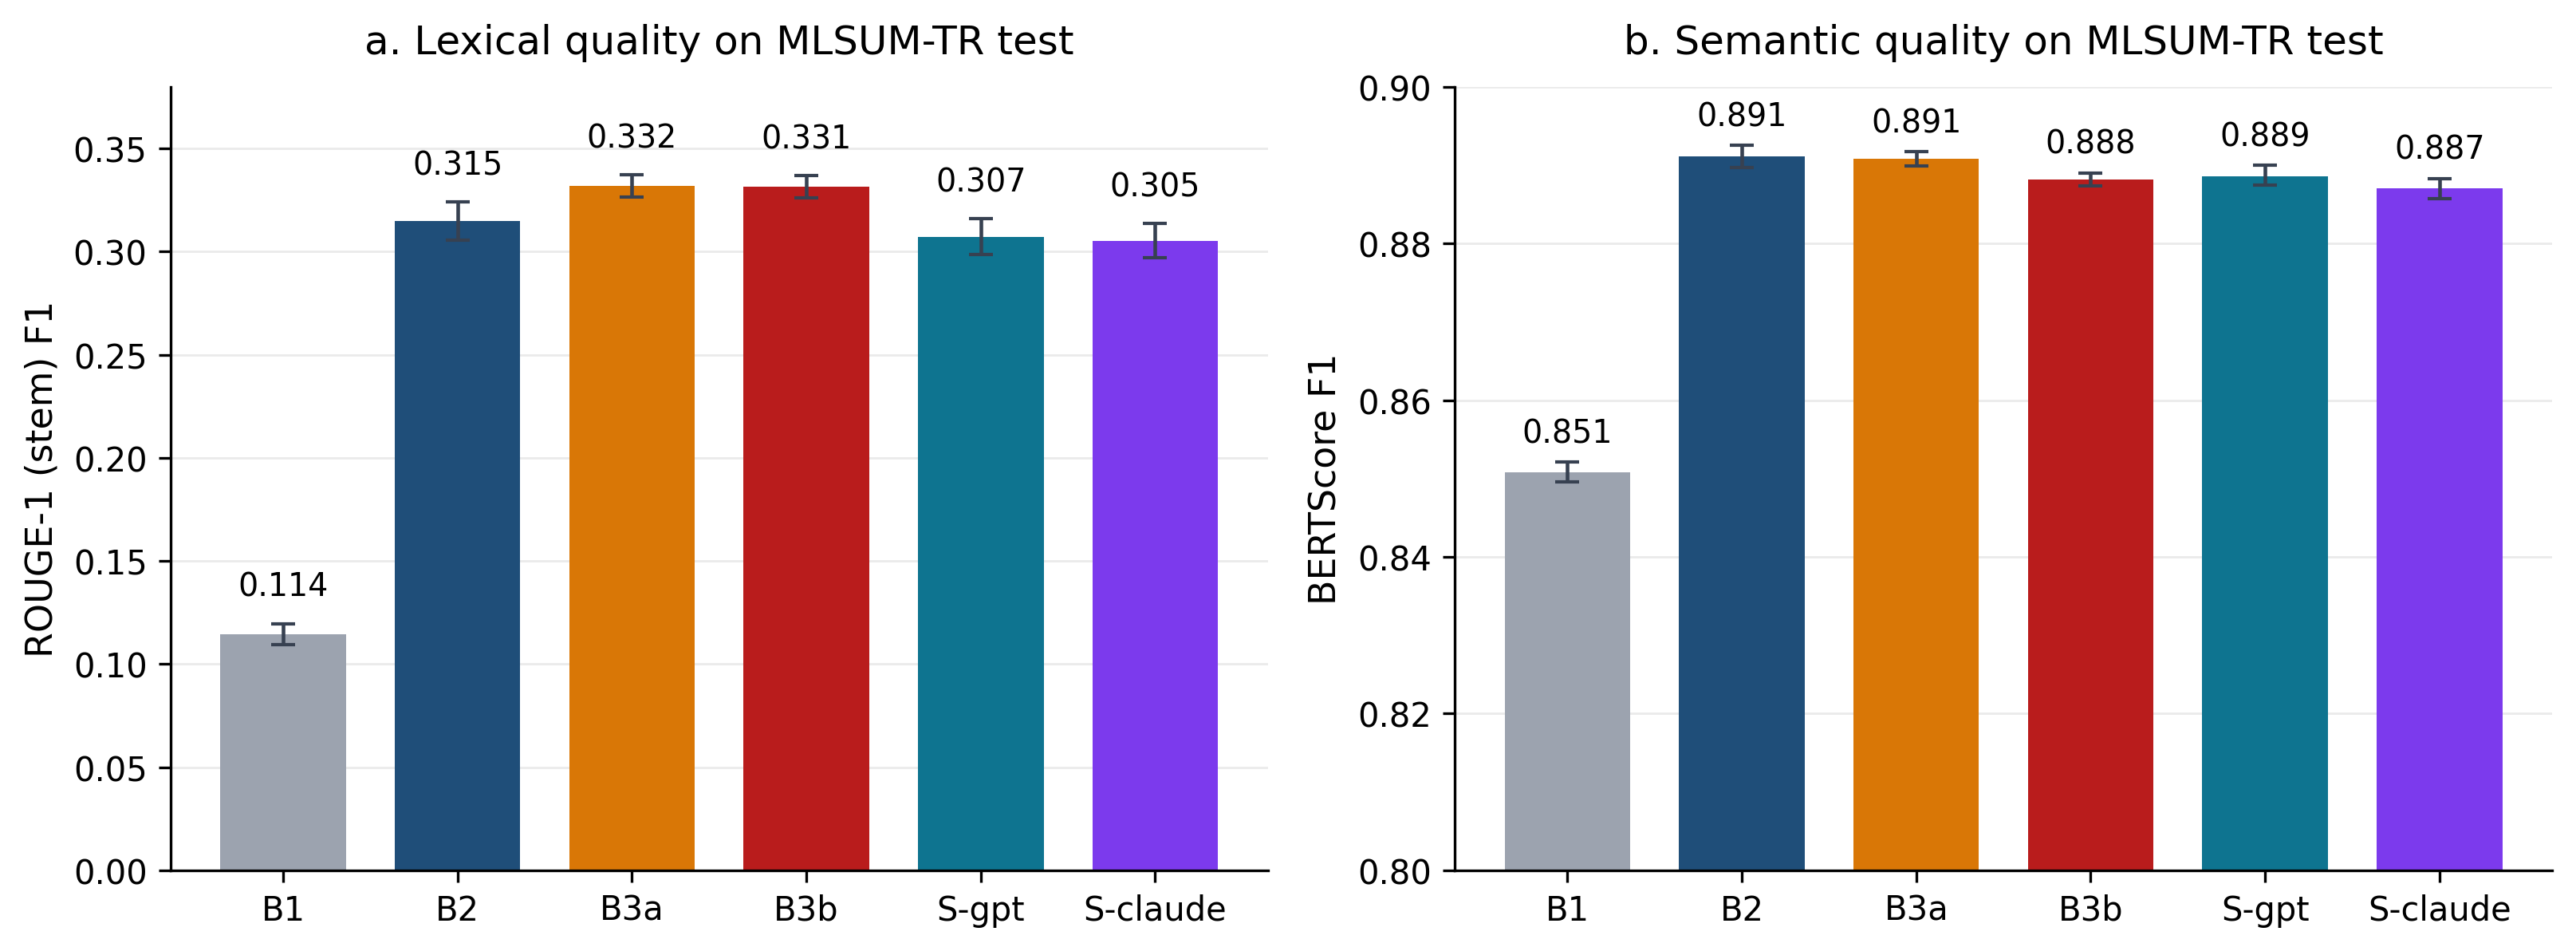
\includegraphics[width=0.92\textwidth]{figures/fig1_main_bar.png}
\caption{Six-system comparison on MLSUM-TR, scored on sentinel-stripped output; error bars are 95\% bootstrap confidence intervals. (a)~ROUGE-1 stem rewards lexical agreement with the reference; teachers and synthetic students both reach $\sim$0.31--0.33. (b)~BERTScore F1 rewards semantic similarity, and here the teachers no longer lead: B3a reaches 0.891, the human-supervised B2 0.891, and the distilled S-gpt 0.889. The $\sim$0.02 gap we reported before stripping the sentinels was an artifact of the decoder output, not a semantic deficit.}
\label{fig:main}
\end{figure*}

\subsection{Out-of-Domain Generalization}
Table~\ref{tab:ood} and Fig.~\ref{fig:ood} report TR-News results. The striking finding: the synthetic students degrade by at most 0.5 R1 points moving out of domain, while the teachers degrade by 2.8--3.2 R1 points. As a consequence, the distilled S-gpt \emph{significantly} outperforms both teachers on TR-News (0.267 vs.\ 0.246 for B3a, $p{=}0.0015$; vs.\ 0.248 for B3b, $p{=}0.0024$; Holm-corrected paired randomization), and it overtakes them on BERTScore F1 as well (0.891 vs.\ 0.889 and 0.887). The mechanism is plausibly that the LLM teachers overfit to MLSUM-style in-distribution patterns the small student never had the capacity to memorize; the student internalizes a more universal extractive prior. This is the strongest argument in favor of distillation here: a 300M-parameter student is both more robust and an order of magnitude cheaper than the LLM it was distilled from. The in-domain equivalence of the two students does not, however, survive the domain shift: out of domain S-gpt exceeds S-claude by $+0.0076$ R1~std with a 90\% CI of $[+0.0023,+0.0129]$, which leaves the $\pm0.010$ margin, so equivalence is \emph{not} established (TOST $p{=}0.23$). Teacher choice appears immaterial in-domain but may matter under distribution shift---a distinction the in-domain comparison alone would have hidden.

\begin{table}[t]
\centering
\caption{Out-of-domain results on TR-News test (1{,}000 articles), on sentinel-stripped output. $\Delta$R1: change versus the in-domain MLSUM-TR result of the same system. Bracketed values are 95\% BCa bootstrap confidence intervals.}
\label{tab:ood}
\footnotesize
\setlength{\tabcolsep}{3pt}
\begin{tabular}{lccccccc}
\toprule
System & R1 std & 95\% CI & R1 stem & BSf1 & halluc\# & lr & $\Delta$R1 \\
\midrule
B1 zero-shot mT5    & 0.096 & [0.089, 0.104] & 0.119 & 0.854 & 0.021 & 0.38 & $+0.002$ \\
B2 human-supervised & \textbf{0.279} & [0.266, 0.292] & \textbf{0.325} & \textbf{0.893} & 0.002 & 1.00 & $+0.002$ \\
B3a GPT-4o-mini     & 0.246 & [0.239, 0.254] & 0.296 & 0.889 & 0.020 & 3.04 & $-0.032$ \\
B3b Claude Haiku 4.5 & 0.248 & [0.241, 0.255] & 0.300 & 0.887 & 0.035 & 3.07 & $-0.028$ \\
S-gpt (synthetic)   & 0.267 & [0.255, 0.280] & 0.314 & 0.891 & \textbf{0.001} & 1.10 & $+0.000$ \\
S-claude (synthetic) & 0.260 & [0.248, 0.271] & 0.304 & 0.888 & 0.006 & 1.37 & $-0.005$ \\
\bottomrule
\end{tabular}
\end{table}

\begin{figure}[t]
\centering
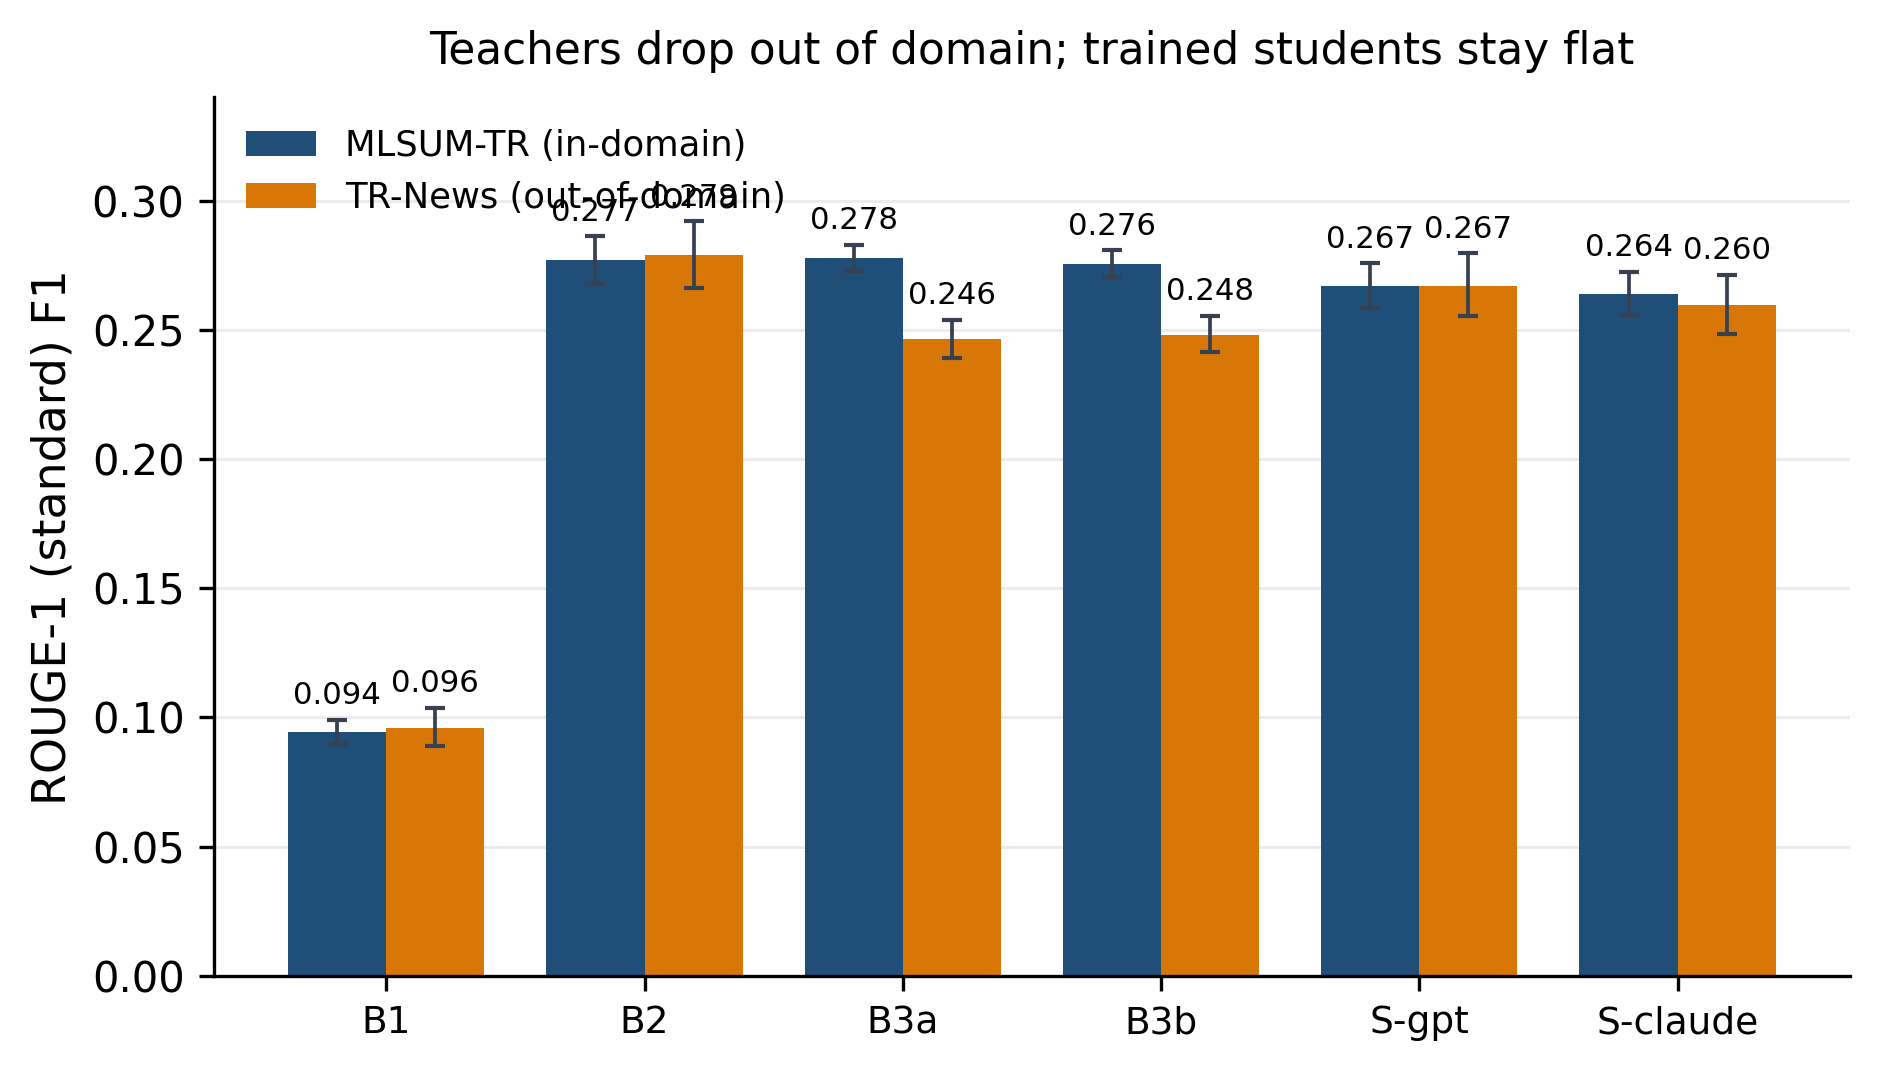
\includegraphics[width=\columnwidth]{figures/fig4_ood.png}
\caption{In-domain vs.\ out-of-domain ROUGE-1 per system, with 95\% bootstrap confidence intervals. Teachers degrade 2.8--3.2 points moving from MLSUM-TR to TR-News; trained students stay flat, and S-gpt overtakes both teachers.}
\label{fig:ood}
\end{figure}

\subsection{Positioning Relative to Prior Turkish Systems}
\label{sec:sota}
Table~\ref{tab:sota} situates our systems against published Turkish abstractive-summarization results on the same corpora. Larger fully-supervised models reach ROUGE-1 in the low 0.40s: on MLSUM-TR, Baykara and Güngör~\cite{baykara2022trnews} report 0.423 for mT5-Base and 0.405 for mBART, the Mukayese mT5-Base~\cite{safaya2022mukayese} reaches a comparable range, and the Turkish-specific TURNA~\cite{uludogan2024turna} and VBART~\cite{turker2024vbart} report further gains. Our 300M distilled student ($\sim$0.31 stemmed ROUGE-1) and even the zero-shot LLM teachers ($\sim$0.33) sit below these.

This gap is expected and instructive rather than a deficiency. First, those systems are roughly twice the size and are fully supervised on the entire training set with untruncated inputs, whereas we use a 300M student, 512-token inputs, 10k synthetic pairs, and a 2{,}000-article test subset. Second, cross-study ROUGE is only indicative: tokenization, stemming, and test splits differ across papers, so absolute values are not directly comparable. Third, in-domain ROUGE rewards reference-style matching, on which even strong zero-shot LLMs underperform a model supervised on that exact distribution. Our contribution is orthogonal to this leaderboard: a distilled student that approaches its own teachers at a fraction of their size and cost, generalizes better out-of-domain (Table~\ref{tab:ood}), and hallucinates substantially less (Section~\ref{sec:errors}), all properties that ROUGE does not capture.

\begin{table}[t]
\centering
\caption{Our systems vs.\ published Turkish summarization results on MLSUM-TR. Prior numbers are as reported by their authors (full test set, their own stemmed ROUGE, full supervision) and are indicative only, not directly comparable; our rows use 5-character-stem ROUGE-1 on the 2{,}000-article subset.}
\label{tab:sota}
\footnotesize
\setlength{\tabcolsep}{4pt}
\begin{tabular}{llcc}
\toprule
System & Params & Supervision & ROUGE-1 \\
\midrule
mT5-Base~\cite{baykara2022trnews}  & 580M & full & 0.423 \\
BERT2BERT~\cite{baykara2022trnews} & $\sim$220M & full & 0.415 \\
mBART25~\cite{baykara2022trnews}   & 610M & full & 0.405 \\
\midrule
B3a GPT-4o-mini (teacher) & --   & zero-shot   & 0.332 \\
B2 mT5-small (human-sup.) & 300M & full (10k)  & 0.315 \\
S-gpt (ours, distilled)   & 300M & 10k synth.  & 0.307 \\
\bottomrule
\end{tabular}
\end{table}

\section{Ablations}
\label{sec:ablations}
We run four ablations along the dimensions most likely to affect the result.

\textbf{Synthetic dataset size.} As the synthetic training set grows from 1k to 10k, R1~std climbs from 0.162 to 0.267 with clear diminishing returns: doubling from 5k to 10k yields only $+3.1$ points after $4\times$ data buys $+7.4$ points going 1k to 5k. The 1k variant exhibits a qualitative \emph{phase transition}: at 1k the student is still in a teacher-mimic regime ($\mathrm{len\_ratio}{=}2.33$, $\mathrm{halluc\#}{=}0.051$), but by 5k it has settled into the compact extractive style ($\mathrm{len\_ratio}{=}0.78$, $\mathrm{halluc\#}{=}0.010$ in this ablation sweep) that it keeps at 10k, where the separate main run in Table~\ref{tab:main} records an even lower $\mathrm{halluc\#}{=}0.004$. The transition is not about learning more facts; it is about adopting the small-model output prior.

\textbf{LoRA rank.} R1~std climbs monotonically with rank: 0.249~(r4) $\to$ 0.267~(r8) $\to$ 0.281~(r16) $\to$ 0.290~(r32). At rank 32 the student \emph{exceeds} the GPT teacher on standard ROUGE-1 (0.290 vs.\ 0.278), but hallucinations rise from 0.003 at rank 16 to 0.012 at rank 32 (a factor of four). The extra capacity appears to memorize teacher-specific tokens, including some of the teacher's hallucinated numbers. Rank 8 is the Pareto-efficient operating point: within 2.3 points of rank 32 on R1, with no hallucination penalty, at one-quarter the trainable parameter count. This recommendation rests on the hallucination trade-off rather than on a quality difference; with single-seed runs we cannot exclude that ranks 8 and 16 differ only by training noise.

\textbf{Prompt design and teacher choice.} Holding size at 1{,}000 synthetic examples, the detailed prompt (which explicitly requires five-W coverage) yields $+1.4$ R1~std points over the concise prompt for the S-gpt student, but the hallucinated-number rate rises by $+1.7$ percentage points (from 0.051 to 0.068): the detailed prompt elicits more specific facts, which the student then over-applies when source evidence is absent. By contrast, comparing S-gpt and S-claude at all matched configurations, the largest in-domain difference is 0.003 R1~std, and the two are statistically equivalent within the pre-registered margin. In-domain, the choice of teacher LLM does not measurably affect downstream student quality; out of domain the equivalence does not hold (Section~\ref{sec:sota} above and Table~\ref{tab:ood}).

\section{Error Analysis}
\label{sec:errors}
\subsection{Heuristic Quantitative Analysis}
Fig.~\ref{fig:halluc} plots ROUGE-1 against hallucinated-number fraction for all six systems on MLSUM-TR. Trained students (B2, S-gpt, S-claude) cluster in the desirable high-quality / low-hallucination quadrant; teachers (B3a, B3b) achieve comparable quality at $\sim$5$\times$ higher hallucination rates; B1 is poor on both. This is the strongest two-dimensional summary of the paper's findings. The flag counts only numeric tokens and is a per-summary rate, so it is confounded with length; Section~\ref{sec:ethics} states what that does and does not license us to claim.

\begin{figure}[t]
\centering
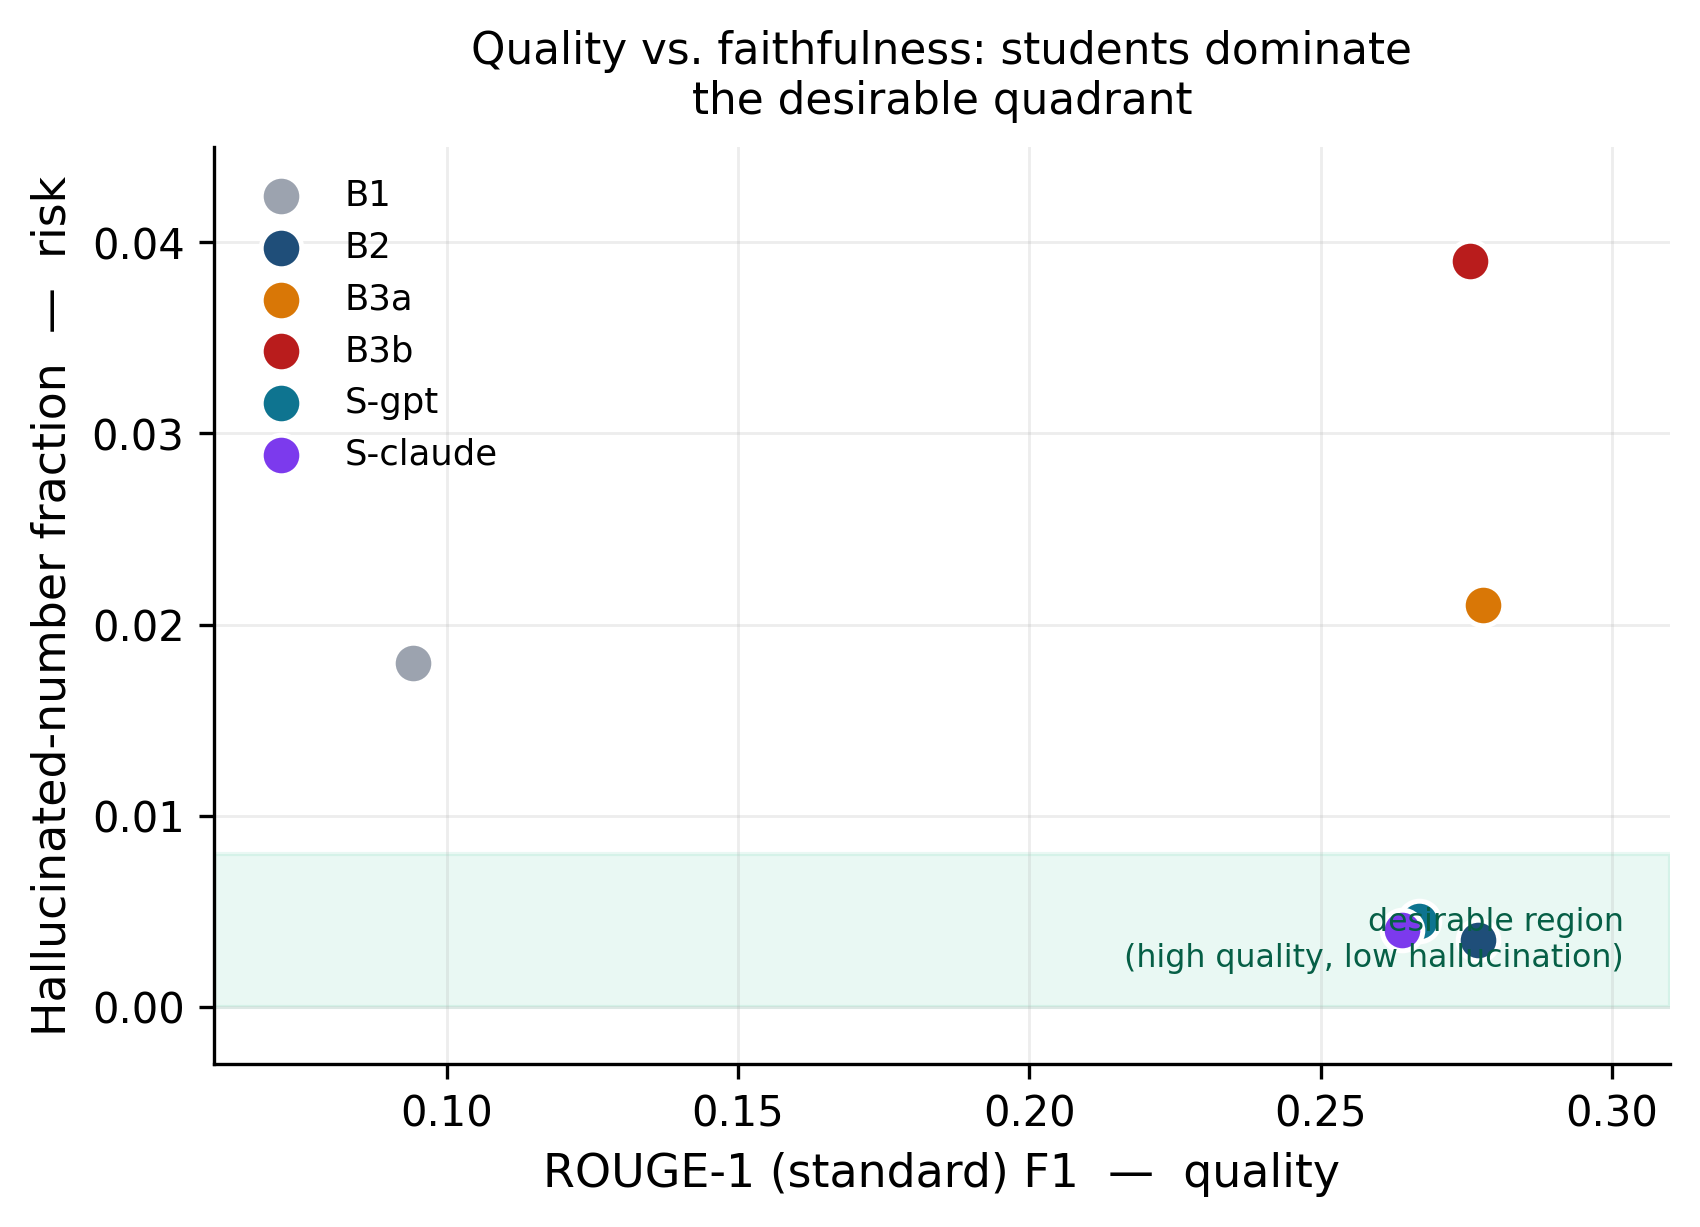
\includegraphics[width=0.86\columnwidth]{figures/fig5_halluc_quality.png}
\caption{Quality (ROUGE-1) versus faithfulness risk (hallucinated-number rate), on sentinel-stripped output. Trained students dominate the desirable bottom-right region; teachers achieve similar quality at $\sim$5$\times$ higher risk. The risk axis counts numeric tokens only and is not length-normalised.}
\label{fig:halluc}
\end{figure}

\subsection{LLM-as-a-Judge Qualitative Analysis}
We sample 30 articles stratified by source length (10 short, 10 medium, 10 long) and score every system's output on five binary axes (factual correctness, completeness, Turkish fluency, morphological correctness, absence of mode collapse), yielding $30 \times 6 = 180$ labeled (article, system) pairs. The labeler is Claude Opus~4.7 acting as judge, following the LLM-as-a-judge methodology of Zheng et al.~\cite{zheng2023judging}. The rubric is biased \emph{strict} on factuality (default to 0 when in doubt) and \emph{lenient} on morphology (default to 1) to compensate for the judge's weaker morphological grounding in Turkish.

The headline pattern (Table~\ref{tab:qual}) is consistent across axes: the GPT-4o-mini teacher (B3a) passes uniformly, while all four small-model systems (B1, B2, S-gpt, S-claude) cluster at 0--3\% fluency pass rate despite ROUGE scores only a few points below the teachers.

\textbf{The fluency gap is a single, fixable decoding artifact, not a content deficiency.} The judge's free-text notes attribute the small-model fluency failures to one recurring cause: the dominant note phrase is ``fragment with \texttt{extra\_id} token'' (74 of 180 rows, 41\%). The mT5 SentencePiece tokenizer reserves sentinel tokens \texttt{<extra\_id\_0>}\,$\dots$\,\texttt{<extra\_id\_99>} for its span-corruption pretraining objective, and these leaked into the \emph{cached} generations scored here when they were not stripped during decoding. We remove them with a one-line regular expression (\texttt{<extra\_id\_\textbackslash d+>}) that is now applied in our released inference code and in every analysis in this paper.

\textbf{The artifact is fully systematic, and it was not confined to fluency.} Contrary to what we assumed when we first found it, the lexical metrics are \emph{not} immune. Our ROUGE tokenizer strips non-word characters, so \texttt{<extra\_id\_0>} loses its angle brackets but survives as the word token \texttt{extra\_id\_0} (and as \texttt{extra} under the 5-character stemmer). Because mT5 is pretrained on span corruption alone, every training target begins with the first sentinel and the decoder reproduces it on \textbf{100\% of small-model outputs}---exactly one occurrence per summary for B2, S-gpt, S-claude and every LoRA and data-size variant, and 1.07 per summary for the untrained B1, whose surplus is genuine span-corruption behaviour. The two API teachers are unaffected, which gives a free internal control. Re-scoring the stripped predictions leaves ROUGE \emph{recall} unchanged to four decimals for every system while raising precision by 1.4--2.9 points; ROUGE-1 F1 rises 0.5--0.7 points and BERTScore F1 by 1.6--2.6 points for the four affected systems, and by exactly zero for the teachers. All deltas exclude zero under a paired bootstrap, and no prediction is emptied by stripping. Every number in Tables~\ref{tab:main}--\ref{tab:sota} and Section~\ref{sec:ablations} is reported on stripped output.

We verified that post-hoc stripping is identical to regenerating with the fixed decoder: decoding 200 articles twice from the same checkpoint, once with and once without the strip, the regular expression applied to the unstripped output reproduced the stripped output on \textbf{198 of 198} comparable rows. The affected content is otherwise sound (factual correctness 83--97\% on the very same outputs), so the fluency column of Table~\ref{tab:qual} reflects pre-strip text and \emph{understates} the deployed system, which emits clean Turkish once the sentinels are removed. We report the pre-strip judge scores unchanged, for transparency; re-running the qualitative evaluation on stripped output is the most important piece of work this revision could not complete (Section~\ref{sec:ethics}).

\textbf{Recurring failure modes.} Beyond the sentinel artifact (74/180 rows), the judge's notes attribute remaining issues to mid-sentence truncation at the token cap (11), non-summary boilerplate fragments (7), and rare teacher hallucinations (e.g.\ a ``George Clooney'' mention not in source). The sentinel issue dominates and, being a decoding-time problem rather than a learned behavior, is fully resolved by the post-processing strip.

\begin{table}[t]
\centering
\caption{Qualitative pass rates from Claude Opus~4.7 as LLM-as-a-judge, on 30 stratified articles $\times$ 6 systems = 180 labeled rows. Each axis is scored 0/1. Overall is the unweighted mean across the five axes. Fluency reflects pre-strip outputs (see text).}
\label{tab:qual}
\footnotesize
\setlength{\tabcolsep}{4pt}
\begin{tabular}{lcccccc}
\toprule
System & Fact. & Compl. & Flu. & Morph. & NoColl. & Overall \\
\midrule
B1 zero-shot mT5    & 0.97 & 0.03 & 0.03 & 1.00 & 0.93 & 0.59 \\
B2 human-supervised & 0.97 & 0.33 & 0.03 & 1.00 & 1.00 & 0.67 \\
B3a GPT-4o-mini     & \textbf{1.00} & \textbf{1.00} & \textbf{1.00} & 1.00 & 1.00 & \textbf{1.00} \\
B3b Claude Haiku 4.5 & 0.97 & 1.00 & 0.63 & 1.00 & 1.00 & 0.92 \\
S-gpt (synthetic)   & 0.90 & 0.57 & 0.00 & 0.97 & 0.97 & 0.68 \\
S-claude (synthetic) & 0.83 & 0.67 & 0.03 & 0.93 & 0.97 & 0.69 \\
\bottomrule
\end{tabular}
\end{table}

\section{Ethics and Limitations}
\label{sec:ethics}
\subsection{Measured Social and Representational Bias}
Because the pipeline ships LLM-generated text into a deployable Turkish summarizer, we quantify three bias dimensions \emph{post hoc} on the existing 2{,}000-article MLSUM-TR predictions, with no retraining. Following Blodgett et al.~\cite{blodgett2020bias}, we treat ``bias'' as a measurable representational harm, and document it as urged for deployable language technology by Bender et al.~\cite{bender2021parrots}: (i)~\emph{gender representation}, the female share of gendered person-mentions (Turkish gendered nouns/honorifics plus a first-name$\rightarrow$gender lexicon), compared against the source articles and human references; (ii)~\emph{foreign-token leakage}, the share of summaries carrying $\geq$1 non-Turkish token (the Turkish alphabet has no \texttt{q}, \texttt{w}, or \texttt{x}, an orthographic signal for English/loanword intrusion); and (iii)~\emph{representational-harm errors} from the 180 LLM-judge notes, categorized by type. Results are in Table~\ref{tab:bias}.

\begin{table}[t]
\centering
\caption{Post-hoc bias metrics on MLSUM-TR test. Fem.\ share: female fraction of gendered mentions (source 0.244, human references 0.215). $\Delta$src: minus the source share. Foreign: \% of summaries with $\geq$1 non-Turkish token. Ident.: identity/attribution errors among 30 judged outputs. Compl.: completeness pass rate.}
\label{tab:bias}
\footnotesize
\setlength{\tabcolsep}{4pt}
\begin{tabular}{lccccc}
\toprule
System & Fem. & $\Delta$src & Foreign & Ident. & Compl. \\
\midrule
B1 zero-shot mT5     & 0.163 & $-0.081$ & 1.6\% & 0 & 0.03 \\
B2 human-supervised  & 0.207 & $-0.037$ & 4.7\% & 0 & 0.33 \\
B3a GPT-4o-mini      & 0.240 & $-0.004$ & 7.9\% & 0 & \textbf{1.00} \\
B3b Claude Haiku 4.5 & \textbf{0.241} & $-0.003$ & 9.5\% & 0 & \textbf{1.00} \\
S-gpt (synthetic)    & 0.206 & $-0.038$ & 5.2\% & 2 & 0.57 \\
S-claude (synthetic) & 0.202 & $-0.042$ & 6.1\% & \textbf{6} & 0.67 \\
\bottomrule
\end{tabular}
\end{table}

\textbf{Gender skew is corpus-rooted and amplified by compression, not by distillation.} MLSUM-TR is heavily male-skewed: only 24.4\% of gendered person-mentions in the source articles are female, and the human references already lower this to 21.5\%. The abstractive teachers almost exactly preserve the source ratio (0.240, 0.241), whereas every \emph{compressive} system (the human-supervised B2 and both distilled students) under-represents women by $\sim$4 points relative to the source (0.202--0.207), landing at or just below the human-reference level (Fig.~\ref{fig:gender}). The distilled students therefore do \emph{not} introduce gender skew beyond what the human gold summaries already exhibit; the effect is driven by aggressive compression (extractive overlap $\approx$0.99, length ratio $\approx$0.8--0.9) dropping secondary actors, who are disproportionately women in this corpus.

\begin{figure}[t]
\centering
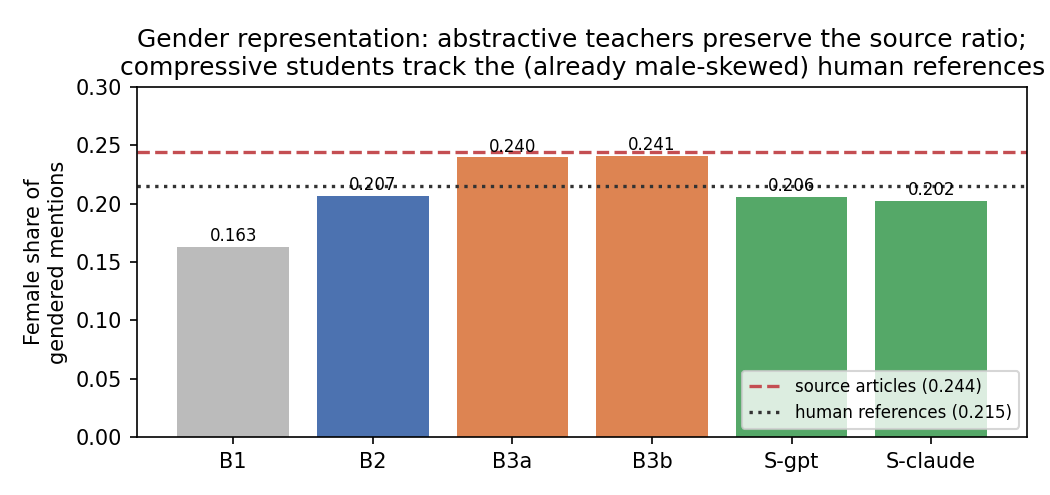
\includegraphics[width=\columnwidth]{figures/fig6_bias_gender.png}
\caption{Female share of gendered mentions per system against the source-article ratio (0.244, dashed) and the human-reference ratio (0.215, dotted). Verbose teachers preserve the source balance; compressive small models track the already-skewed references.}
\label{fig:gender}
\end{figure}

\textbf{Cultural/English leakage is real but bounded, and distillation reduces it.} GPT-4o-mini and Claude Haiku~4.5 emit a foreign token in 7.9\% and 9.5\% of summaries respectively, versus 5.2--6.1\% for the distilled students and 4.7\% for the human-supervised baseline. Token-level density is uniformly low ($\sim$2--3 foreign tokens per 1{,}000) and most flagged tokens are legitimate foreign \emph{named entities} present in the source (e.g.\ \emph{Twitter}, \emph{Volkswagen}, \emph{NHS}) rather than gratuitous English. The distilled students leak less than their teachers because their extractive prior keeps them anchored to the Turkish source text.

\textbf{Representational-harm errors concentrate in the students.} Identity/attribution errors (wrong subject, misattributed action, swapped or misspelled named entities, confused country) appear \emph{only} in the distilled students (S-gpt 2/30, S-claude 6/30) and in none of the baselines or teachers (Fig.~\ref{fig:repharm}); S-claude's factual-correctness pass rate falls to 0.83. These are the highest-harm class for a news summarizer, since they can attribute an action or crime to the wrong named person. They share a mechanism with the gendered omission above: aggressive compression under a 300M-parameter budget garbles \emph{who did what} and drops secondary participants. The same compression that cuts numeric hallucination five-fold thus trades one faithfulness risk (fabrication) for two others (omission and misattribution), and the omission is not gender-neutral.

\begin{figure}[t]
\centering
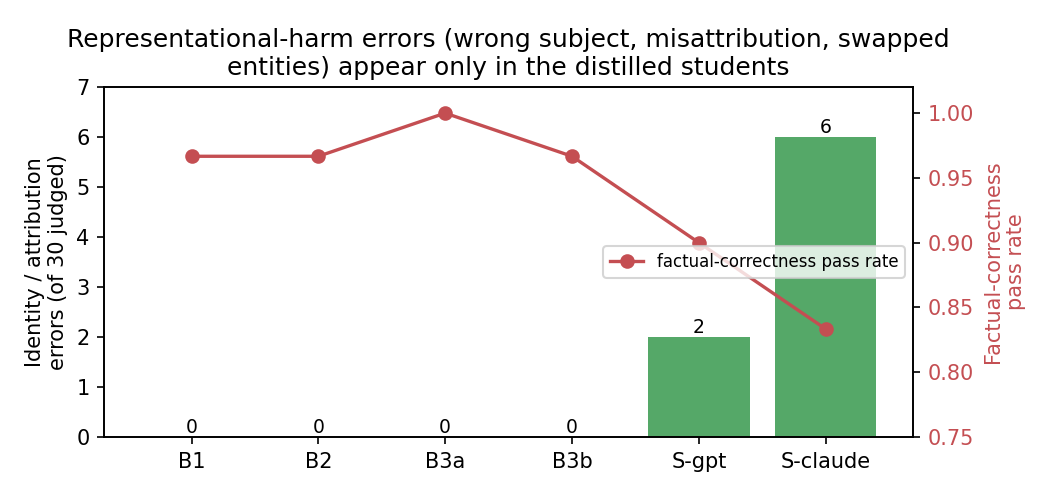
\includegraphics[width=\columnwidth]{figures/fig8_bias_repharm.png}
\caption{Identity/attribution errors among the 30 judged outputs per system (bars) and factual-correctness pass rate (line). Such errors are absent from the teachers and baselines and appear only after distillation into the small student.}
\label{fig:repharm}
\end{figure}

\textbf{Mitigations.} We (i)~strip mT5 \texttt{<extra\_id\_*>} sentinels before release and evaluation; (ii)~withhold public release of student weights given both the synthetic-news misuse risk and the elevated misattribution rate; (iii)~recommend that any deployment touching named individuals retain human review or an entity-consistency check, since neither ROUGE nor BERTScore detects misattribution; and (iv)~note that the gender skew could be reduced by re-balancing the synthetic corpus toward female-salient articles. Topic-stratified fairness could not be measured because the loaded MLSUM-TR records carried no usable topic field; extending the probe across news categories is left to future work.

\subsection{Evaluation and Model Limitations}
ROUGE on Turkish systematically underestimates quality due to agglutinative-morphology fragmentation; BERTScore captures semantics but cannot detect hallucinated facts (a fluent confident lie scores high), so the qualitative analysis is essential to any deployment recommendation. Our use of mT5-small is a deliberate constraint of the free-tier T4 (15~GB) budget rather than a modeling recommendation: mT5-small is the largest mT5 that fits with LoRA on this hardware. Larger students (mT5-base/large, mBART-50, mT0) would raise the quality ceiling and are the natural next step; that said, the per-parameter out-of-domain robustness reported above suggests the small student already generalizes beyond its size. The one substantive output artifact, SentencePiece sentinel leakage, is a decoding-time issue resolved by the post-processing strip now in the released code, not a limitation of the distillation method itself.

Four further limitations should be stated plainly rather than left to inference.

\textbf{Single training run.} Every trained system is one run at seed 42. The intervals above capture test-set sampling uncertainty only, not training-seed variance, so the equivalence results hold for \emph{these particular runs} on this test set. A three-seed protocol (seeds 42/1337/2024 for B2, S-gpt and S-claude, and for LoRA ranks 16 and 32) is implemented and pre-registered in the repository but was not executed before the camera-ready deadline.

\textbf{Judge independence.} The labels in Table~\ref{tab:qual} come from a single Claude model, and Claude Haiku~4.5 both generated B3b's summaries and supervised S-claude, so the judge is not independent of two of the six systems it scores. The judge prompt also carried the system label and only the first 600 characters of the source article while asking for a strict factuality verdict. A blinded protocol with a 3{,}000-character context and two non-Anthropic judges is implemented in the repository; running it, together with the pre- versus post-strip contrast, is the first item of future work.

\textbf{Faithfulness is measured on numbers only.} The \texttt{halluc\#} flag checks whether a numeric token in the summary appears in the source. It says nothing about fabricated or misattributed persons, events and relations, which for a news summarizer are the higher-harm class, and it is confounded with length: the teachers write 2.1--3.1$\times$ the reference length and the students 0.7--1.4$\times$, so a per-summary rate mechanically favours the shorter system. The five-fold figure should be read as a length-uncontrolled, numeric-only estimate. Entity-level precision and recall, length-normalised rates, and a human-annotated misattribution axis are specified in the repository but not yet measured.

\textbf{Omission is partly architectural.} The student's 512-token input window covers the median MLSUM-TR article (1{,}159 characters) but not the tail (p95 4{,}061; maximum 26{,}612). Some of what reads as omission is content the student never saw.

\subsection{Reproducibility}
All prompts, training configurations, evaluation scripts, per-example scores, the statistical analysis code, and the pre-registration of the equivalence margin are publicly available at \url{https://github.com/cagancaliskan/turkish-summarization-distillation}. Total experimental cost was approximately \$15 in API fees plus approximately 14 hours of T4 GPU time on Colab.

\section{Conclusion}
A small student model (mT5-small + LoRA rank 8) trained on 10{,}000 synthetic summaries from a commercial LLM teacher matches the teacher within 1.1 ROUGE-1 points in-domain, significantly outperforms both teachers by 1.9--2.1 R1 points out-of-domain on TR-News, hallucinates approximately five times fewer numeric facts, and runs at a fraction of the inference cost. The teacher comparison is an equivalence result in-domain, established by TOST at a pre-registered $\pm0.010$ margin rather than by a failure to reject: GPT-4o-mini and Claude Haiku~4.5 are interchangeable as zero-shot summarizers and, in-domain, as distillation supervisors. Ablations show that quality is bounded by the size of the synthetic supervision rather than by LoRA capacity; rank 8 is Pareto-optimal because higher ranks improve ROUGE only at the cost of faithfulness, though single-seed runs cannot separate ranks 8 and 16 from training noise. The strongest case for distillation is out-of-domain robustness: the small student learns a more universal extractive prior than the LLM it was distilled from.

\footnotesize
\begin{thebibliography}{00}
\bibitem{scialom2020mlsum} T. Scialom, P.-A. Dray, S. Lamprier, B. Piwowarski, and J. Staiano, ``MLSUM: The multilingual summarization corpus,'' in \emph{Proc. EMNLP}, 2020, pp. 8051--8067.
\bibitem{baykara2022trnews} B. Baykara and T. Güngör, ``Abstractive text summarization and new large-scale datasets for agglutinative languages: Turkish and Hungarian,'' \emph{Lang. Resour. Eval.}, vol. 56, pp. 973--1007, 2022.
\bibitem{xue2021mt5} L. Xue \emph{et al.}, ``mT5: A massively multilingual pre-trained text-to-text transformer,'' in \emph{Proc. NAACL-HLT}, 2021, pp. 483--498.
\bibitem{hu2021lora} E. J. Hu \emph{et al.}, ``LoRA: Low-rank adaptation of large language models,'' in \emph{Proc. ICLR}, 2022.
\bibitem{hinton2015distillation} G. Hinton, O. Vinyals, and J. Dean, ``Distilling the knowledge in a neural network,'' \emph{arXiv:1503.02531}, 2015.
\bibitem{taori2023alpaca} R. Taori \emph{et al.}, ``Stanford Alpaca: An instruction-following LLaMA model,'' Stanford CRFM, 2023.
\bibitem{wang2023selfinstruct} Y. Wang \emph{et al.}, ``Self-Instruct: Aligning language models with self-generated instructions,'' in \emph{Proc. ACL}, 2023, pp. 13484--13508.
\bibitem{lin2004rouge} C.-Y. Lin, ``ROUGE: A package for automatic evaluation of summaries,'' in \emph{Text Summarization Branches Out}, 2004, pp. 74--81.
\bibitem{zhang2020bertscore} T. Zhang, V. Kishore, F. Wu, K. Q. Weinberger, and Y. Artzi, ``BERTScore: Evaluating text generation with BERT,'' in \emph{Proc. ICLR}, 2020.
\bibitem{zheng2023judging} L. Zheng \emph{et al.}, ``Judging LLM-as-a-judge with MT-Bench and Chatbot Arena,'' in \emph{Proc. NeurIPS Datasets and Benchmarks}, 2023.
\bibitem{blodgett2020bias} S. L. Blodgett, S. Barocas, H. Daumé III, and H. Wallach, ``Language (technology) is power: A critical survey of `bias' in NLP,'' in \emph{Proc. ACL}, 2020, pp. 5454--5476.
\bibitem{bender2021parrots} E. M. Bender, T. Gebru, A. McMillan-Major, and S. Shmitchell, ``On the dangers of stochastic parrots: Can language models be too big?'' in \emph{Proc. FAccT}, 2021, pp. 610--623.
\bibitem{see2017pointer} A. See, P. J. Liu, and C. D. Manning, ``Get to the point: Summarization with pointer-generator networks,'' in \emph{Proc. ACL}, 2017, pp. 1073--1083.
\bibitem{lewis2020bart} M. Lewis, Y. Liu, N. Goyal, M. Ghazvininejad, A. Mohamed, O. Levy, V. Stoyanov, and L. Zettlemoyer, ``BART: Denoising sequence-to-sequence pre-training for natural language generation, translation, and comprehension,'' in \emph{Proc. ACL}, 2020, pp. 7871--7880.
\bibitem{raffel2020t5} C. Raffel, N. Shazeer, A. Roberts, K. Lee, S. Narang, M. Matena, Y. Zhou, W. Li, and P. J. Liu, ``Exploring the limits of transfer learning with a unified text-to-text transformer,'' \emph{J. Mach. Learn. Res.}, vol. 21, no. 140, pp. 1--67, 2020.
\bibitem{zhang2020pegasus} J. Zhang, Y. Zhao, M. Saleh, and P. J. Liu, ``PEGASUS: Pre-training with extracted gap-sentences for abstractive summarization,'' in \emph{Proc. ICML}, 2020, pp. 11328--11339.
\bibitem{liu2020mbart} Y. Liu, J. Gu, N. Goyal, X. Li, S. Edunov, M. Ghazvininejad, M. Lewis, and L. Zettlemoyer, ``Multilingual denoising pre-training for neural machine translation,'' \emph{Trans. Assoc. Comput. Linguistics}, vol. 8, pp. 726--742, 2020.
\bibitem{safaya2022mukayese} A. Safaya, E. Kurtulu\c{s}, A. G\"okto\u{g}an, and D. Yuret, ``Mukayese: {T}urkish {NLP} strikes back,'' in \emph{Findings of the ACL}, 2022, pp. 846--863.
\bibitem{uludogan2024turna} G. Uludo\u{g}an, Z. Y. Balal, F. Akkurt, M. Turker, O. G\"ung\"or, and S. \"Usk\"udarl\i, ``{TURNA}: A {T}urkish encoder-decoder language model for enhanced understanding and generation,'' in \emph{Findings of the ACL}, 2024, pp. 10103--10117.
\bibitem{turker2024vbart} M. T\"urker, M. E. Ar\i, and A. Han, ``{VBART}: The {T}urkish {LLM},'' \emph{arXiv:2403.01308}, 2024.
\bibitem{schweter2020berturk} S. Schweter, ``{BERTurk}: {BERT} models for {T}urkish,'' Zenodo, 2020, doi: 10.5281/zenodo.3770924.
\bibitem{kim2016seqkd} Y. Kim and A. M. Rush, ``Sequence-level knowledge distillation,'' in \emph{Proc. EMNLP}, 2016, pp. 1317--1327.
\bibitem{shleifer2020distilbart} S. Shleifer and A. M. Rush, ``Pre-trained summarization distillation,'' \emph{arXiv:2010.13002}, 2020.
\bibitem{hsieh2023distilling} C.-Y. Hsieh, C.-L. Li, C.-K. Yeh, H. Nakhost, Y. Fujii, A. Ratner, R. Krishna, C.-Y. Lee, and T. Pfister, ``Distilling step-by-step! Outperforming larger language models with less training data and smaller model sizes,'' in \emph{Findings of the ACL}, 2023, pp. 8003--8017.
\bibitem{houlsby2019adapters} N. Houlsby, A. Giurgiu, S. Jastrzebski, B. Morrone, Q. de Laroussilhe, A. Gesmundo, M. Attariyan, and S. Gelly, ``Parameter-efficient transfer learning for NLP,'' in \emph{Proc. ICML}, 2019, pp. 2790--2799.
\bibitem{dettmers2023qlora} T. Dettmers, A. Pagnoni, A. Holtzman, and L. Zettlemoyer, ``{QLoRA}: Efficient finetuning of quantized {LLMs},'' in \emph{Proc. NeurIPS}, 2023.
\bibitem{maynez2020faithfulness} J. Maynez, S. Narayan, B. Bohnet, and R. McDonald, ``On faithfulness and factuality in abstractive summarization,'' in \emph{Proc. ACL}, 2020, pp. 1906--1919.
\bibitem{lakens2017equivalence} D. Lakens, ``Equivalence tests: A practical primer for $t$-tests, correlations, and meta-analyses,'' \emph{Soc. Psychol. Personal. Sci.}, vol. 8, no. 4, pp. 355--362, 2017.
\bibitem{dror2018hitchhiker} R. Dror, G. Baumer, S. Shlomov, and R. Reichart, ``The hitchhiker's guide to testing statistical significance in natural language processing,'' in \emph{Proc. ACL}, 2018, pp. 1383--1392.
\bibitem{kryscinski2020factcc} W. Kry\'sci\'nski, B. McCann, C. Xiong, and R. Socher, ``Evaluating the factual consistency of abstractive text summarization,'' in \emph{Proc. EMNLP}, 2020, pp. 9332--9346.
\end{thebibliography}

\end{document}